\documentclass{article}
\usepackage[utf8]{inputenc}
\usepackage[T1]{fontenc}
\usepackage[utf8]{inputenc}
\usepackage{lmodern}
\usepackage[a4paper, margin=1in]{geometry}
\usepackage{graphicx}
\usepackage[section]{placeins}
\usepackage{minted}
\large
\title{ECE9603 Final Report}
\begin{document}
\begin{titlepage}
	\begin{center}
    \line(1,0){300}\\
    [0.65cm]
	\huge{\bfseries Final Report}\\
	\line(1,0){300}\\
	\textsc{\Large ECE9603: Data Analytics}\\
	\textsc{\LARGE \today}\\
	[5.5cm]     
	\end{center}
	\begin{center}
		\textsc{\Large Names}\\
		\textsc{\Large Names}\\
		\textsc{\Large Names}\\
		\textsc{\Large Names}\\
		[0.75cm]
	\end{center}
\end{titlepage}

\section*{Methodology - Established (FFNN and SVM)}
\subsection*{Data Preparation}
The dataset consisted of muscle activity readings for 8 sensors which measured the electrical activity produced by muscle movement. Each line consisted of 8 consecutive readings for all 8 sensors, yielding 64 columns of EMG data plus a target column for the gesture. The data was fairly balanced across all gestures, with each gesture occupying 2900 lines of data. Each 1x64 row was reformatted by stacking corresponding sensor readings on top of each other, transforming each entry into an 8x8 matrix. Doing so allowed each row to represent one time step for all 8 sensors. A target column was appended to each entry for each corresponding gesture. Data was recorded at 200 Hz, meaning that each line represented 40ms of muscle activity readings. Our review of studies in the related work found that data is often divided into segments and analyzed in time windows. These windows can either be contiguous or overlapping \textbf{[Figure X]}. The optimal window length for upper-limb myoelectric devices is within the range of 150-250 ms \textbf{[REFERENCE NUMBER]}. We chose a window duration of 200 ms with an overlap of 50 ms. This resulted in an average of 777 windows generated between all four gestures. 

\begin{figure}[!htb]
\caption{EMG Signal with overlapping windows}
\centering
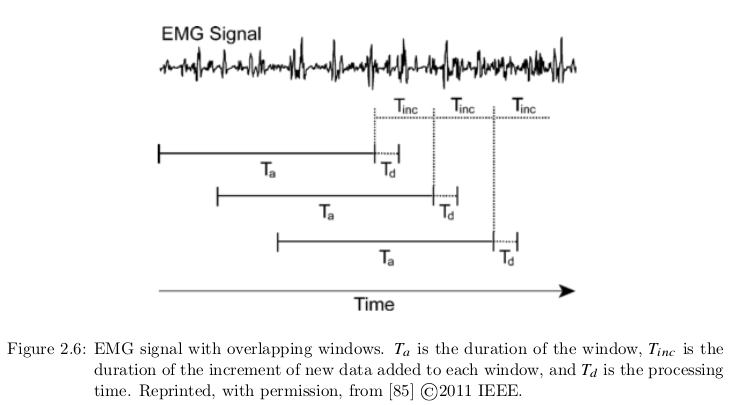
\includegraphics[scale=0.5]{Images/EMG_Signal.png}
\end{figure}

For the neural networks, the gestures were encoded in one-hot format such that a softmax activation function could be used for the output layer. The SVM left the target classes in their numerical form 0 through 3. The data was randomly split 60/20/20 into training, validation, and testing data. The networks were tuned using the validation and testing data, and then after the network parameters were finalized, it was tested with the test data for comparison amongst the three types of networks created. 

\subsection*{Feature Extraction}
After the data is windowed, several features are computed for each windowed section to increase the total number of attributes and obtain additional information from the EMG data. There are many options for the time-domain features that can be obtained, but the four most popular options were selected. Each feature is computed for each of the 8 data sensors, resulting in a total of 56 attributes.

\subsubsection*{Mean Absolute Value (MAV)} To compute the MAV, the absolute values are taken for each reading, then averaged across each window, as illustrated in Equation 1, where \(x_n(i)\) is the reading for channel n at time i, and m is the window size.

\begin{center}
Equation 1: MAV Feature Calculation
\[ MAV(n) = \frac{1}{m}\sum_{i=1}^{m}\left|(x_n(i)\right| \]
\end{center}

\subsubsection*{Waveform Length (WL)} This feature states the cumulative length of the signal, as per Equation 2, where N is the length of the signal and x(i) is the ith sample of the signal.
\begin{center}
Equation 2: WL Feature Calculation
\[ WL = \sum_{i=1}^{N-1}\left|(x(i+1) - x(i)\right| \]
\end{center}

\subsubsection*{Zero Crossing (ZC)}
This feature counts the number of times the signal crosses zero.

\subsubsection*{Auto-Regressive Coefficients (AR)}
Each channel is represented by a \(4^{th}\) order AR model and the features are the coefficients for the model. The coefficients can be computed using Equation 3, where $P$ is the AR order, $ap$ are the AR coefficients, and \(w_i\) is a white noise term.
\begin{center}
Equation 3: AR Equation
\[ x_i = \sum_{p=1}^{P}a_px_{i-p}+w_i \]
\end{center}

\subsection*{SVM}
A Support Vector Classifier (SVC) was used to approximate the decision boundaries between the four gesture classes. Four hyperparameters were tuned during training. An L2 regularization parameter $C$ was introduced to prevent the model from overfitting. A kernel parameter specified which kernel to use during computation and offered a variety of paths the model could take towards finding suitable decision boundaries. For instance, the linear kernel would only be effective at finding linearly separable decision boundaries whereas the polynomial and RBF kernels are especially useful when the data points are not linearly separable. When the polynomial kernel function is used, the degree of the polynomial is specified by the 'degree' hyperparameter. Similarly, the 'gamma' parameter specifies the kernel coefficients for the RBF, polynomial and sigmoid functions. The values of the hyperparameters space are given below.

\begin{figure}[!htb]
\caption{SVM Hyperparameter Tuning Space}
\begin{table}[H]
\centering
\begin{tabular}{|l|l|}
\hline
\multicolumn{1}{|c|}{\textbf{Hyperparameter}} & \multicolumn{1}{c|}{\textbf{Options}} \\ \hline
C              & 1, 10, 100, 1000                  \\ \hline
Kernel         & 'Linear', 'Poly', 'RBF', Sigmoid' \\ \hline
Degree         & 1, 3, 5, 7                        \\ \hline
Gamma          & 'Scale', 'Auto'                   \\ \hline
\end{tabular}
\end{table}
\end{figure}

A baseline SVC model was instantiated with the default parameters \{‘C’: 1, 'kernel': linear, 'gamma': 'scale'\} which was then fit on the training data. 10-fold cross validation was used to obtain a baseline train score. GridSearchCV was applied to search over the hyperparameter space given in the table above. GridSearchCV exhausted all possible combinations of parameters looking for the model yielding the best 10-fold cross validation accuracy score. Once obtained, the selected model was evaluated on the test set for final results.

\subsection*{FFNN}
A simple fully connected FFNN was created to distinguish the gestures from each other. The input layer had 56 neurons as there are 56 features being input into the network, and the output layer had four neurons to support the softmax activation function for the last layer. L2 regularization was used in all layers to help prevent overfitting. The number of hidden layers and the number of neurons in the hidden layer were tuned using the default parameters for the all other hyperparameters. The loss functions of these networks were observed to determine the number of epochs that should be used for fine tuning the network. The range of neurons in the hidden layer were computed using Equation 4 where $a$ was varied from 4 to 10 to attempt to prevent overfitting \textbf{[REFERENCE - http://hagan.okstate.edu/NNDesign.pdf\#page=469]}. This resulted in using 4, 6, and 8 neurons in the hidden layers.

\begin{center}
Equation 4: Number of neurons per hidden layer 
    \[ \textit{\# Neurons in hidden layer} = \frac{\textit{\# Data points in training set}}{a*(\textit{\# Neurons in input layer + \# Layers in output layer})} \]
\end{center}

After the network structure was settled, the learning rate, learning function, and activation function were tuned in a grid search. \textbf{[FIGURE XX]} summarizes the options investigated for the hyperparameters that were tuned. Default parameters were used for all other options. The models for tuning were evaluated using the accuracy evaluation metric. After completing the hyperparameter tuning, the best model was evaluated on the test data. 

\begin{figure}[!htb]
\caption{FFNN Hyperparameter Tuning Space}
\begin{table}[H]
\centering
\begin{tabular}{|l|l|}
\hline
\multicolumn{1}{|c|}{\textbf{Hyperparameter}} & \multicolumn{1}{c|}{\textbf{Options}} \\ \hline
Number of Hidden layers            & 0, 1, 2                         \\ \hline
Number of Neurons in hidden layers & 4, 6, 8                         \\ \hline
Learning Function                  & 'Adam', 'SGD'                   \\ \hline
Learning rate                      & 0.001,0.01,0.05,0.1,0.2,0.3,0.4 \\ \hline
Activation function                & 'ReLU', 'ELU', 'Sigmoid'        \\ \hline
\end{tabular}
\end{table}
\end{figure}

\section*{Methodology - Novel (LSTM)}
\subsection*{Data Preparation}
EMG data from each gesture was divided into sliding windows of 200 ms and 50 ms overlap. Then, each window was stacked on top of each other horizontally to form a 3D array that was going to be used to train the LSTM network. Each row of the 3D array represented a training sample, whereas each column represented the EMG reading of one of the eight channels/sensors of the Myo Armband. The third dimension of the 3D array represented the lag values of each EMG sensor/channel. After creating a 3D array for each gesture, the rows of this 3D array were randomly shuffled and then were divided into the training set, the cross-validation set, and the testing set, each one having 60\%, 20\%, and 20\%, respectively, of the whole gesture dataset. This procedure was repeated for each of the remaining gesture datasets. Having divided the data into the three sets, the data labels were separated and then, one-hot encoding was used on the data labels in order for them to be classified using a softmax activation function. 

\subsection*{LSTM}
LSTM networks have been widely used in sequence problems where there exists a time dependency between data points. They have become popularized for being able to retain information over longer periods of time, a problem that traditional RNNs have struggled with. A baseline LSTM model was constructed with a 50-unit LSTM layer which then passed through a dropout layer, dropping 20\% of the neurons. The remaining neurons were fed into a 100-unit dense layer with the ReLU activation function. In order to output classes, the dense layer was connected to a 4-unit softmax layer which outputted gesture classifications. Tuning took place on the number of hidden dense layers, the number of neurons per hidden layer, the activation function and the dropout rate. The values of the hyperparameter space are given below.

\begin{figure}[!htb]
\caption{LSTM Hyperparameter Tuning Space}
\begin{table}[H]
\centering
\begin{tabular}{|l|l|}
\hline
\multicolumn{1}{|c|}{\textbf{Hyperparameter}} & \multicolumn{1}{c|}{\textbf{Options}} \\ \hline
Number of Hidden layers            & 0, 1, 2                            \\ \hline
Number of Neurons in hidden layers & 4, 6, 8                            \\ \hline
Activation function                & 'ReLU', 'ELU', 'Sigmoid'           \\ \hline
Dropout rate                       & 0.15, 0.18, 0.21, 0.24, 0.27, 0.30 \\ \hline
\end{tabular}
\end{table}
\end{figure}

A baseline LSTM model was instantiated with the parameters \{‘\# Hidden layers’: 1,  ‘\# Neurons per layer’: 100, ‘Activation function’: ReLU, ‘Dropout rate’: \} which was then fit on the training data. Hold out cross validation was used to obtain a baseline train score. During tuning, RandomSearch randomly sampled a set of parameters from the available parameters and returned the model yielding the lowest hold out validation score. The selected model was then evaluated on the test set for final results.

\section*{Results}
\subsection*{Evaluation Metrics}
Three metrics were used to evaluate the performance of our models: accuracy, precision and recall. Accuracy was the most important metric since it represents the proportion of true results among the total number of cases examined. Precision was used to examine the proportion of predicted gestures that were actually correct, for each class. Recall was used to evaluate the proportion of actual gestures that were correctly identified by the models. The equations for how we calculated these metrics are given below.

\begin{center}
Evaluation Metrics
    \[ \textrm{Accuracy} = \frac{\textrm{\# Correct predictions}}{\textrm{Total \# predictions}} \]
    \[ \textrm{Precision} = \frac{\textrm{True Positives}}{\textrm{True Positives + False Positives}} \textrm{, per gesture}\]
    \[ \textrm{Recall} = \frac{\textrm{True Positives}}{\textrm{True Positives + False Negatives}} \textrm{, per gesture}\]
\end{center}

\subsection*{SVM Results}
Results after iterating through the hyperparameter space showed that linear and low-order polynomial models performed the best. In general, linear kernels consistently outperformed all other kernels. Almost every single linear kernel, regardless of the state of other hyperparameters, scored an impressive 99.48\% accuracy on the validation set. This was only 0.4\% lower than the highest score, which was found by a 1st-order polynomial kernel with minimal smoothing. Kernels that performed notably worse were the sigmoid and RBF kernels, scoring up to 75\% worse than their peers when all other hyperparameter values were left equal. Regularization appeared to have minimal effect over the polynomial kernels and no effect on linear kernels. The validation score decreased as the degree of the polynomial kernel increased, signalling the data had a strong preference for linear models. The best performing models and their hyperparameters are summarized in \textbf{[Figure ZZ]}. The scores reported are their validation scores. Based on these results, Network 1 was selected to be evaluated on the test set. It scored a test accuracy of 99.36\%. \textbf{[FIGURE XX]} shows the confusion matrix generated the predictions made on the test set by Network 1, and \textbf{[FIGURE XX]} shows the corresponding precision and recall scores.

\begin{figure}[!htb]
\caption{SVM Hyptertuning Results}
\begin{table}[H]
\centering
\begin{tabular}{|l|l|l|l|l|l|}
\hline
\multicolumn{1}{|c|}{\textbf{Hyperparameter}} & \multicolumn{1}{c|}{\textbf{Network 1}} & Network 2               & Network 3               & Network 4               & Network 5               \\ \hline
C                                             & 10                                      & 1                       & 1                       & 1                       & 10                      \\ \hline
Kernel                                        & Polynomial                              & Linear                  & Linear                  & Linear                  & Linear                  \\ \hline
Degree                                        & 1                                       & 1                       & 3                       & 3                       & 1                       \\ \hline
Gamma                                         & Scale                                   & Scale                   & Scale                   & Auto                    & Scale                   \\ \hline
\textit{\textbf{Validation Accuracy}}         & \textit{\textbf{99.52\%}}                 & \textit{\textbf{99.48\%}} & \textit{\textbf{99.48\%}} & \textit{\textbf{99.48\%}} & \textit{\textbf{99.48\%}} \\ \hline
\end{tabular}
\end{table}
\end{figure}

\begin{figure}[!htb]
\caption{SVM Confusion Matrix}
\centering
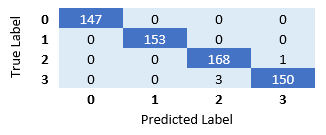
\includegraphics[scale=0.5]{Images/SVM_confusion_matrix.png}
\end{figure}

\begin{figure}[!htb]
\caption{SVM Precision and Recall Scores}
\centering
\includegraphics[scale=0.5]{Images/SVM_prec_rec.png}
\end{figure}

\subsection*{FFNN Results}
Upon investigating which network architecture performed best, the 2-layer network consistently resulted in higher accuracies than the 3- and 4-layer networks, as overfitting was beginning to occur. It was found that the loss function stabilized after approximately 30 epochs, thus 120 epochs were used for all further tuning. The 4-layer networks got “stuck” and would not pass accuracies of 25-35\%, despite trying multiple learning rates and 200+ epochs. The grid search was performed with the 2 layer network and the best performing 3 layer network (4 neurons in the hidden layer) to determine if tuning would improve the performance of the 3 layer network. The best performing models and their hyperparameters are summarized in \textbf{[Figure ZZ]}. Again, it was found that the 2-layer network consistently performed better than the 3-layer one. When the SGD learning function was used, there was no dependency for the model’s accuracy on the learning rate once it was larger than 0.05. On the other hand, with the Adam learning function, the accuracy decreased as the learning rate increased. Additionally, the Adam learning function frequently resulted in a loss function that oscillated about an asymptote, as opposed to converging to the asymptote like the SGD function did. For both learning functions, the number of epoch required for the loss function to reach the asymptote decreased as the learning rate increased. The sigmoid activation function resulted in accuracies around 97-98\%, whereas 99\% accuracy was achieved with both ReLU and ELU activation functions. Overall, Network 1 showed the most promise, scoring an accuracy of 99.36\% on the validation set and an accuracy of 98.71\% on the test set. \textbf{[Figure XX]} displays the confusion matrix for Network 1 on the test data, while \textbf{[Figure XX]} shows the corresponding precision and recall values for each gesture. The rows are what the gesture is, whereas the columns are what the FFNN predicted. The network was capable of identifying gesture 1 with no problems. It struggled more with gestures 3 and 4. Gesture 3 was sometimes mistaken for 2 or 4, whereas gesture 4 was mistaken for all the other options in 1-2 instances.

\begin{figure}[!htb]
\caption{FFNN Hypertuning Results}
\begin{table}[H]
\centering
\begin{tabular}{|l|l|l|l|l|l|}
\hline
\multicolumn{1}{|c|}{\textbf{Hyperparameter}} & \multicolumn{1}{c|}{\textbf{Network 1}} & Network 2               & Network 3               & Network 4               & Network 5               \\ \hline
Number of Hidden layers                       & 2                                       & 2                       & 2                       & 2                       & 3                       \\ \hline
Number of Neurons in hidden layers            & -                                       & -                       & -                       & -                       & 4                       \\ \hline
Learning Function                             & Sgd                                     & Adam                    & Sgd                     & Sgd                     & Sgd                     \\ \hline
Learning rate                                 & 0.05-0.4                                & 0.001                   & 0.05-0.4                & 0.05-0.4                & 0.05-0.4                \\ \hline
Activation function                           & ReLU                                    & ELU                     & ELU                     & Sigmoid                 & Sigmoid                 \\ \hline
\textit{\textbf{Validation Accuracy}}         & \textit{\textbf{99.36}}                 & \textit{\textbf{99.36}} & \textit{\textbf{99.20}} & \textit{\textbf{98.71}} & \textit{\textbf{98.87}} \\ \hline
\end{tabular}
\end{table}
\end{figure}

\begin{figure}[!htb]
\caption{FFNN Confusion Matrix}
\centering
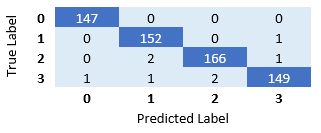
\includegraphics[scale=0.5]{Images/FFNN_confusion_matrix.png}
\end{figure}

\begin{figure}[!htb]
\caption{FFNN Precision and Recall Scores}
\centering
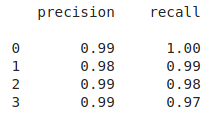
\includegraphics[scale=0.5]{Images/FFNN_prec_rec.png}
\end{figure}

\subsection*{LSTM Results}
After reviewing the results from the RandomSearch hyperparameter tuning process, we found that networks with 3 to 4 hidden layers were consistently preferred, although one shallow network with a single hidden layer performed substantially well. We observed no strong preference for the number of neurons per hidden layer, though it’s worth noting that the highest scoring models tended to have a couple dense layers of 100+ neurons. We also found that having too harsh of a dropout policy negatively affected the models performance. Results show that a dropout rate of 18\%-24\% generated the highest validation scores, with scores dipping drastically after the 27\% mark. Finally, we found that the ELU activation function consistently outperformed the ReLU function and was the activation function of choice for the first 8 out of 10 top models returned by RandomSearch. The best performing models and their hyperparameters are summarized in \textbf{[Figure ZZ]}. The scores reported are their validation scores. Network 1 was evaluated on the test set and scored a test accuracy of 99.36\%. \textbf{[Figure XX]} shows the training accuracy and loss graphs for Network 1, which was selected from RandomSearch. \textbf{[Figure XX]} shows the confusion matrix for Network 1 on the test set. 

\begin{figure}[!htb]
\caption{LSTM Hypertuning Results}
\begin{table}[H]
\centering
\begin{tabular}{|l|l|l|l|l|l|}
\hline
\multicolumn{1}{|c|}{\textbf{Hyperparameter}} & \multicolumn{1}{c|}{\textbf{Network 1}} & Network 2               & Network 3               & Network 4               & Network 5               \\ \hline
Number of Hidden layers                       & 3                                       & 1                       & 3                       & 4                       & 3                       \\ \hline
Number of Neurons in hidden layers            & 50, 200, 200                            & 50                      & 100, 50, 100            & 100, 50, 150, 150       & 150, 150, 200           \\ \hline
Activation function                           & ELU                                     & ELU                     & ELU                     & ELU                     & ELU                     \\ \hline
Dropout rate                                  & 21\%                                    & 24\%                    & 15\%                    & 21\%                    & 18\%                    \\ \hline
\textit{\textbf{Validation Accuracy}}         & \textit{\textbf{99.68}}                 & \textit{\textbf{99.67}} & \textit{\textbf{99.64}} & \textit{\textbf{99.61}} & \textit{\textbf{99.56}} \\ \hline
\end{tabular}
\end{table}
\end{figure}

\begin{figure}[!htb]
\caption{LSTM Training Loss}
\centering
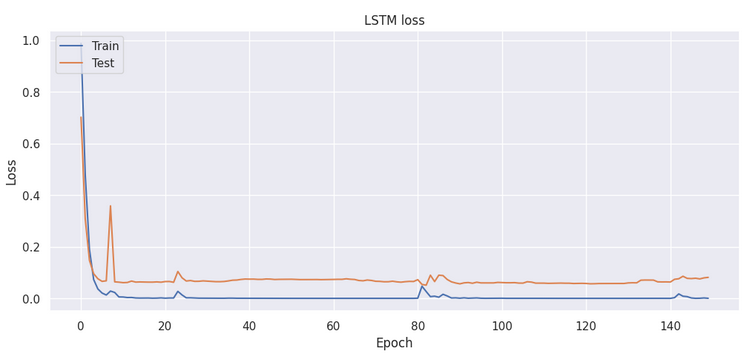
\includegraphics[scale=0.5]{Images/LSTM_train_loss.png}
\end{figure}

\begin{figure}[!htb]
\caption{LSTM Training Accuracy}
\centering
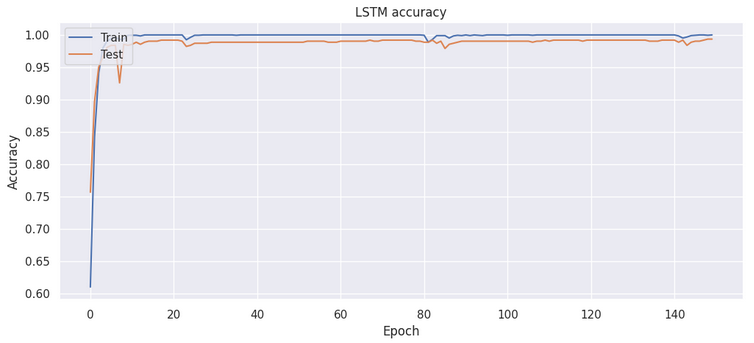
\includegraphics[scale=0.5]{Images/LSTM_train_accuracy.png}
\end{figure}

\begin{figure}[!htb]
\caption{LSTM Confusion Matrix}
\centering
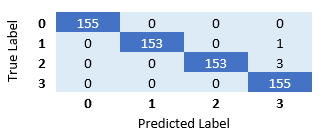
\includegraphics[scale=0.5]{Images/LSTM_confusion_matrix.png}
\end{figure}

\begin{figure}[!htb]
\caption{LSTM Precision and Recall Scores}
\centering
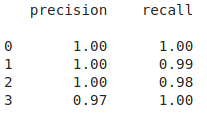
\includegraphics[scale=0.5]{Images/LSTM_prec_rec.png}
\end{figure}

\subsection*{Model Comparison}
\textbf{[Table XX]} summarizes the test accuracy for the three methods. It is clear that all three methods are very successful. Based on the tuning that was performed, the SVM and LSTM networks performed better than the FFNN. While care was taken to tune each network approximately the same amount, it is possible that with further tuning the FFNN could achieve the accuracy obtained by the other two methods. From observing the precision and recall tables, it can be seen that each architecture had issues with different gestures. The novel LSTM neural network mis-identified gesture 2 more than others. It had no issues with gestures 0 or 3. Conversely, the SVM and FFNN had more issues with gesture 3 than the others. This difference could be due to the feature extraction that was performed for the FFNN and the SVM. It is fortunate to know that the LSTM network, once trained, performs comparably to the standard methods. This is advantageous for real-time systems (such as video games for rehabilitation), as they would not have to take the time or computational power to compute all the features while the system is running, which could lead to faster response times.

\begin{figure}[!htb]
\caption{Final Model Comparison}
\begin{table}[H]
\centering
\begin{tabular}{|l|l|l|l|}
\hline
Method                          & SVM                     & FFNN                    & LSTM                    \\ \hline
\textit{\textbf{Test Accuracy}} & \textit{\textbf{99.36}} & \textit{\textbf{99.71}} & \textit{\textbf{99.68}} \\ \hline
\end{tabular}
\end{table}
\end{figure}

\end{document}
